\documentclass[t,xcolor={svgnames,table}]{beamer}

\mode<presentation>
\usetheme{Warsaw}
\useoutertheme{infolines} 
\usepackage{natbib}
\usepackage{fontspec}
\usepackage{lmodern}
\usepackage{amsmath}
\usepackage{amsfonts}
\usepackage{bbm}
\usepackage{bm}
\usepackage[font=small,labelfont=bf]{caption} % Required for specifying captions to tables and figures
\usepackage{nicefrac}
\usepackage{color}
\usepackage{perpage}
\usepackage{multirow}
\usepackage{multicol}
\usepackage{adjustbox}
\usepackage{tikz}
\usepackage{tikz-dependency}
\usepackage{tikz-qtree}
\usepackage{tikz,pgfplots,pgfplotstable}
\usepackage{pgf}
\usepackage{collcell}
\usepackage{booktabs}
\usepackage{color,soul}
\usepackage[absolute,overlay]{textpos}

\usetikzlibrary{arrows.meta,graphs,graphs.standard,graphdrawing,quotes,shapes}
\usegdlibrary{layered,trees}

\tikzset{
  invisible/.style={opacity=0},
  visible on/.style={alt={#1{}{invisible}}},
  alt/.code args={<#1>#2#3}{%
    \alt<#1>{\pgfkeysalso{#2}}{\pgfkeysalso{#3}} % \pgfkeysalso doesn't change the path
  },
}
\captionsetup{labelformat=empty}

\newfontfamily\hebfont[Script=Hebrew, Scale=MatchUppercase]{FreeSans}
\newcommand{\heb}[1]{\bgroup\textdir TRT\hebfont #1\egroup}

\newcommand{\ucca}[1]{\textcolor{gray}{\textbf{\textsf{#1}}}}
\newcommand{\sst}[1]{\textsc{#1}}
\newcommand{\lexcat}[1]{\textsl{#1}}

\definecolor{orange}{rgb}{1,0.5,0}
\definecolor{mdgreen}{rgb}{0.05,0.6,0.05}
\definecolor{Acolor}{HTML}{EC5D57} % poppy red
\definecolor{Pcolor}{HTML}{70BF41} % grass green
\definecolor{Scolor}{HTML}{51A7F9} % sky blue
\definecolor{Lcolor}{HTML}{B36AE2} % friendly purple
\definecolor{mdblue}{rgb}{0,0,0.7}
\definecolor{dkblue}{rgb}{0,0,0.5}
\definecolor{dkgray}{rgb}{0.3,0.3,0.3}
\definecolor{slate}{rgb}{0.25,0.25,0.4}
\definecolor{gray}{rgb}{0.5,0.5,0.5}
\definecolor{ltgray}{rgb}{0.7,0.7,0.7}
\definecolor{purple}{rgb}{0.7,0,1.0}
\definecolor{lavender}{rgb}{0.65,0.55,1.0}


\makeatletter
\pgfdeclareshape{vector}{
      \inheritsavedanchors[from={rectangle}]
      \inheritbackgroundpath[from={rectangle}]
      \inheritanchorborder[from={rectangle}]
      \foreach \x in {center,north east,north west,north,south,south east,south west,east,west}{
        \inheritanchor[from={rectangle}]{\x}
      }

    \backgroundpath{
      \pgftransformshift{\pgfpoint{-16pt}{-4pt}}
          \draw[rounded corners=2pt] (0,0) rectangle (32pt,8pt);
    }

    \beforebackgroundpath{
      \draw[step=8pt,help lines,-] (8pt,.1pt) grid (24pt,7.9pt);
    }
}
\pgfdeclareshape{vector}{
      \inheritsavedanchors[from={rectangle}]
      \inheritbackgroundpath[from={rectangle}]
      \inheritanchorborder[from={rectangle}]
      \foreach \x in {center,north east,north west,north,south,south east,south west,east,west}{
        \inheritanchor[from={rectangle}]{\x}
      }

    \backgroundpath{
      \pgftransformshift{\pgfpoint{-16pt}{-4pt}}
          \draw[rounded corners=2pt] (0,0) rectangle (32pt,8pt);
    }

    \beforebackgroundpath{
      \draw[step=8pt,help lines,-] (8pt,.1pt) grid (24pt,7.9pt);
    }
}
\makeatother


% for confusion matrix
\newcommand{\ApplyGradient}[1]{%
  \pgfmathsetmacro{\PercentColor}{(#1-0)/63.88}%
  \pgfmathsetmacro{\PercentInverse}{ifthenelse(\PercentColor > 70, 0, 100)}%
  %\textcolor{black!\PercentColor}{#1}
  \edef\x{\noexpand\cellcolor{red!\PercentColor}}\x\textcolor{black!\PercentInverse}{#1}%
}
\newcolumntype{R}{>{\collectcell\ApplyGradient}{c}<{\endcollectcell}}


\MakePerPage{footnote}


\begin{document}


\title[]{Meaning Representation and Parsing}
\author{Daniel Hershcovich}
\date{DIKU Bits \\ February 18, 2020}

\begin{frame}
\titlepage
\end{frame}

\begin{frame}
\frametitle{Short Introduction}
\begin{minipage}{.7\textwidth}
2005--2010 \\
\textbf{B.Sc. in Mathematics and Computer Science}, \\
The Open University of Israel
\end{minipage}
\begin{minipage}{.2\textwidth}

\includegraphics[width=\textwidth]{Open_university_israel_logo.png}
\end{minipage}

\vfill\pause

\begin{minipage}{.7\textwidth}
2008--2019 \\
\textbf{Software Engineer} \\
IBM Research
\end{minipage}
\begin{minipage}{.25\textwidth}

\includegraphics[width=\textwidth]{eye_bee_m.png}
\end{minipage}

\vfill\pause

\begin{minipage}{.7\textwidth}
2012--2019 \\
\textbf{Ph.D. in Computational Neuroscience} \\
The Hebrew University of Jerusalem
\end{minipage}
\begin{minipage}{.1\textwidth}

\includegraphics[width=\textwidth]{Hebrew_University_new_Logo_2.png}
\end{minipage}
\end{frame}

\begin{frame}
\frametitle{Short Introduction}
\begin{minipage}{.7\textwidth}
2005--2010 The Open University of Israel
\end{minipage}
\begin{minipage}{.1\textwidth}

\includegraphics[width=\textwidth]{Open_university_israel_logo.png}
\end{minipage}

\vfill

\begin{minipage}{.7\textwidth}
2008--2019 IBM Research
\end{minipage}
\begin{minipage}{.125\textwidth}

\includegraphics[width=\textwidth]{eye_bee_m.png}
\end{minipage}

\vfill

\begin{minipage}{.7\textwidth}
2012--2019 The Hebrew University of Jerusalem
\end{minipage}
\begin{minipage}{.05\textwidth}

\includegraphics[width=\textwidth]{Hebrew_University_new_Logo_2.png}
\end{minipage}

\vfill

\begin{minipage}{.7\textwidth}
Since 2019 \\
University of Copenhagen
\end{minipage}
\begin{minipage}{.2\textwidth}

\includegraphics[width=\textwidth]{ku.png}
\end{minipage}
\end{frame}


\begin{frame}
\frametitle{IBM Project Debater (2012--2019)}

\begin{minipage}{.8\textwidth}
AI system that can debate humans on complex topics \\
(e.g., \textbf{We should ban the sale of violent video games})
\end{minipage}
\begin{minipage}{.125\textwidth}

\includegraphics[width=\textwidth]{eye_bee_m.png}
\end{minipage}

\vfill
\begin{center}

\includegraphics[width=.6\textwidth]{project-debater_resize_md.png}
\end{center}

5 research papers, e.g.,
{\only<2>{\color{red}}
\hfill \textit{Context Dependent Claim Detection} (2014)
}

\only<2>{
\begin{textblock*}{64mm}(32mm,0.34\textheight)
\begin{exampleblock}{}
Because violence in video games is interactive and not passive, critics such as Dave
Grossman and Jack Thompson argue that \textbf{violence in games hardens children to
unethical acts}, calling first-person shooter games ``murder simulators'', although
no conclusive evidence has supported this belief
\end{exampleblock}
\end{textblock*}}

\vfill

{\only<3>{\color{red}}
\hfill \textit{Argument Invention from First Principles} (2019)
}

\only<3>{
\begin{textblock*}{64mm}(32mm,0.34\textheight)
\begin{exampleblock}{}
\textbf{Freedom of choice} $\to$ People have the right to make their own choices, including bad ones \vspace{6mm}

\textbf{Black market} $\to$ Prohibiting products and activities makes them less visible and available, and thus less harmful
\end{exampleblock}
\end{textblock*}}
\end{frame}

\begin{frame}
\setbeamercovered{transparent}
\frametitle{What can we teach computers to do with language?}
\only<5>{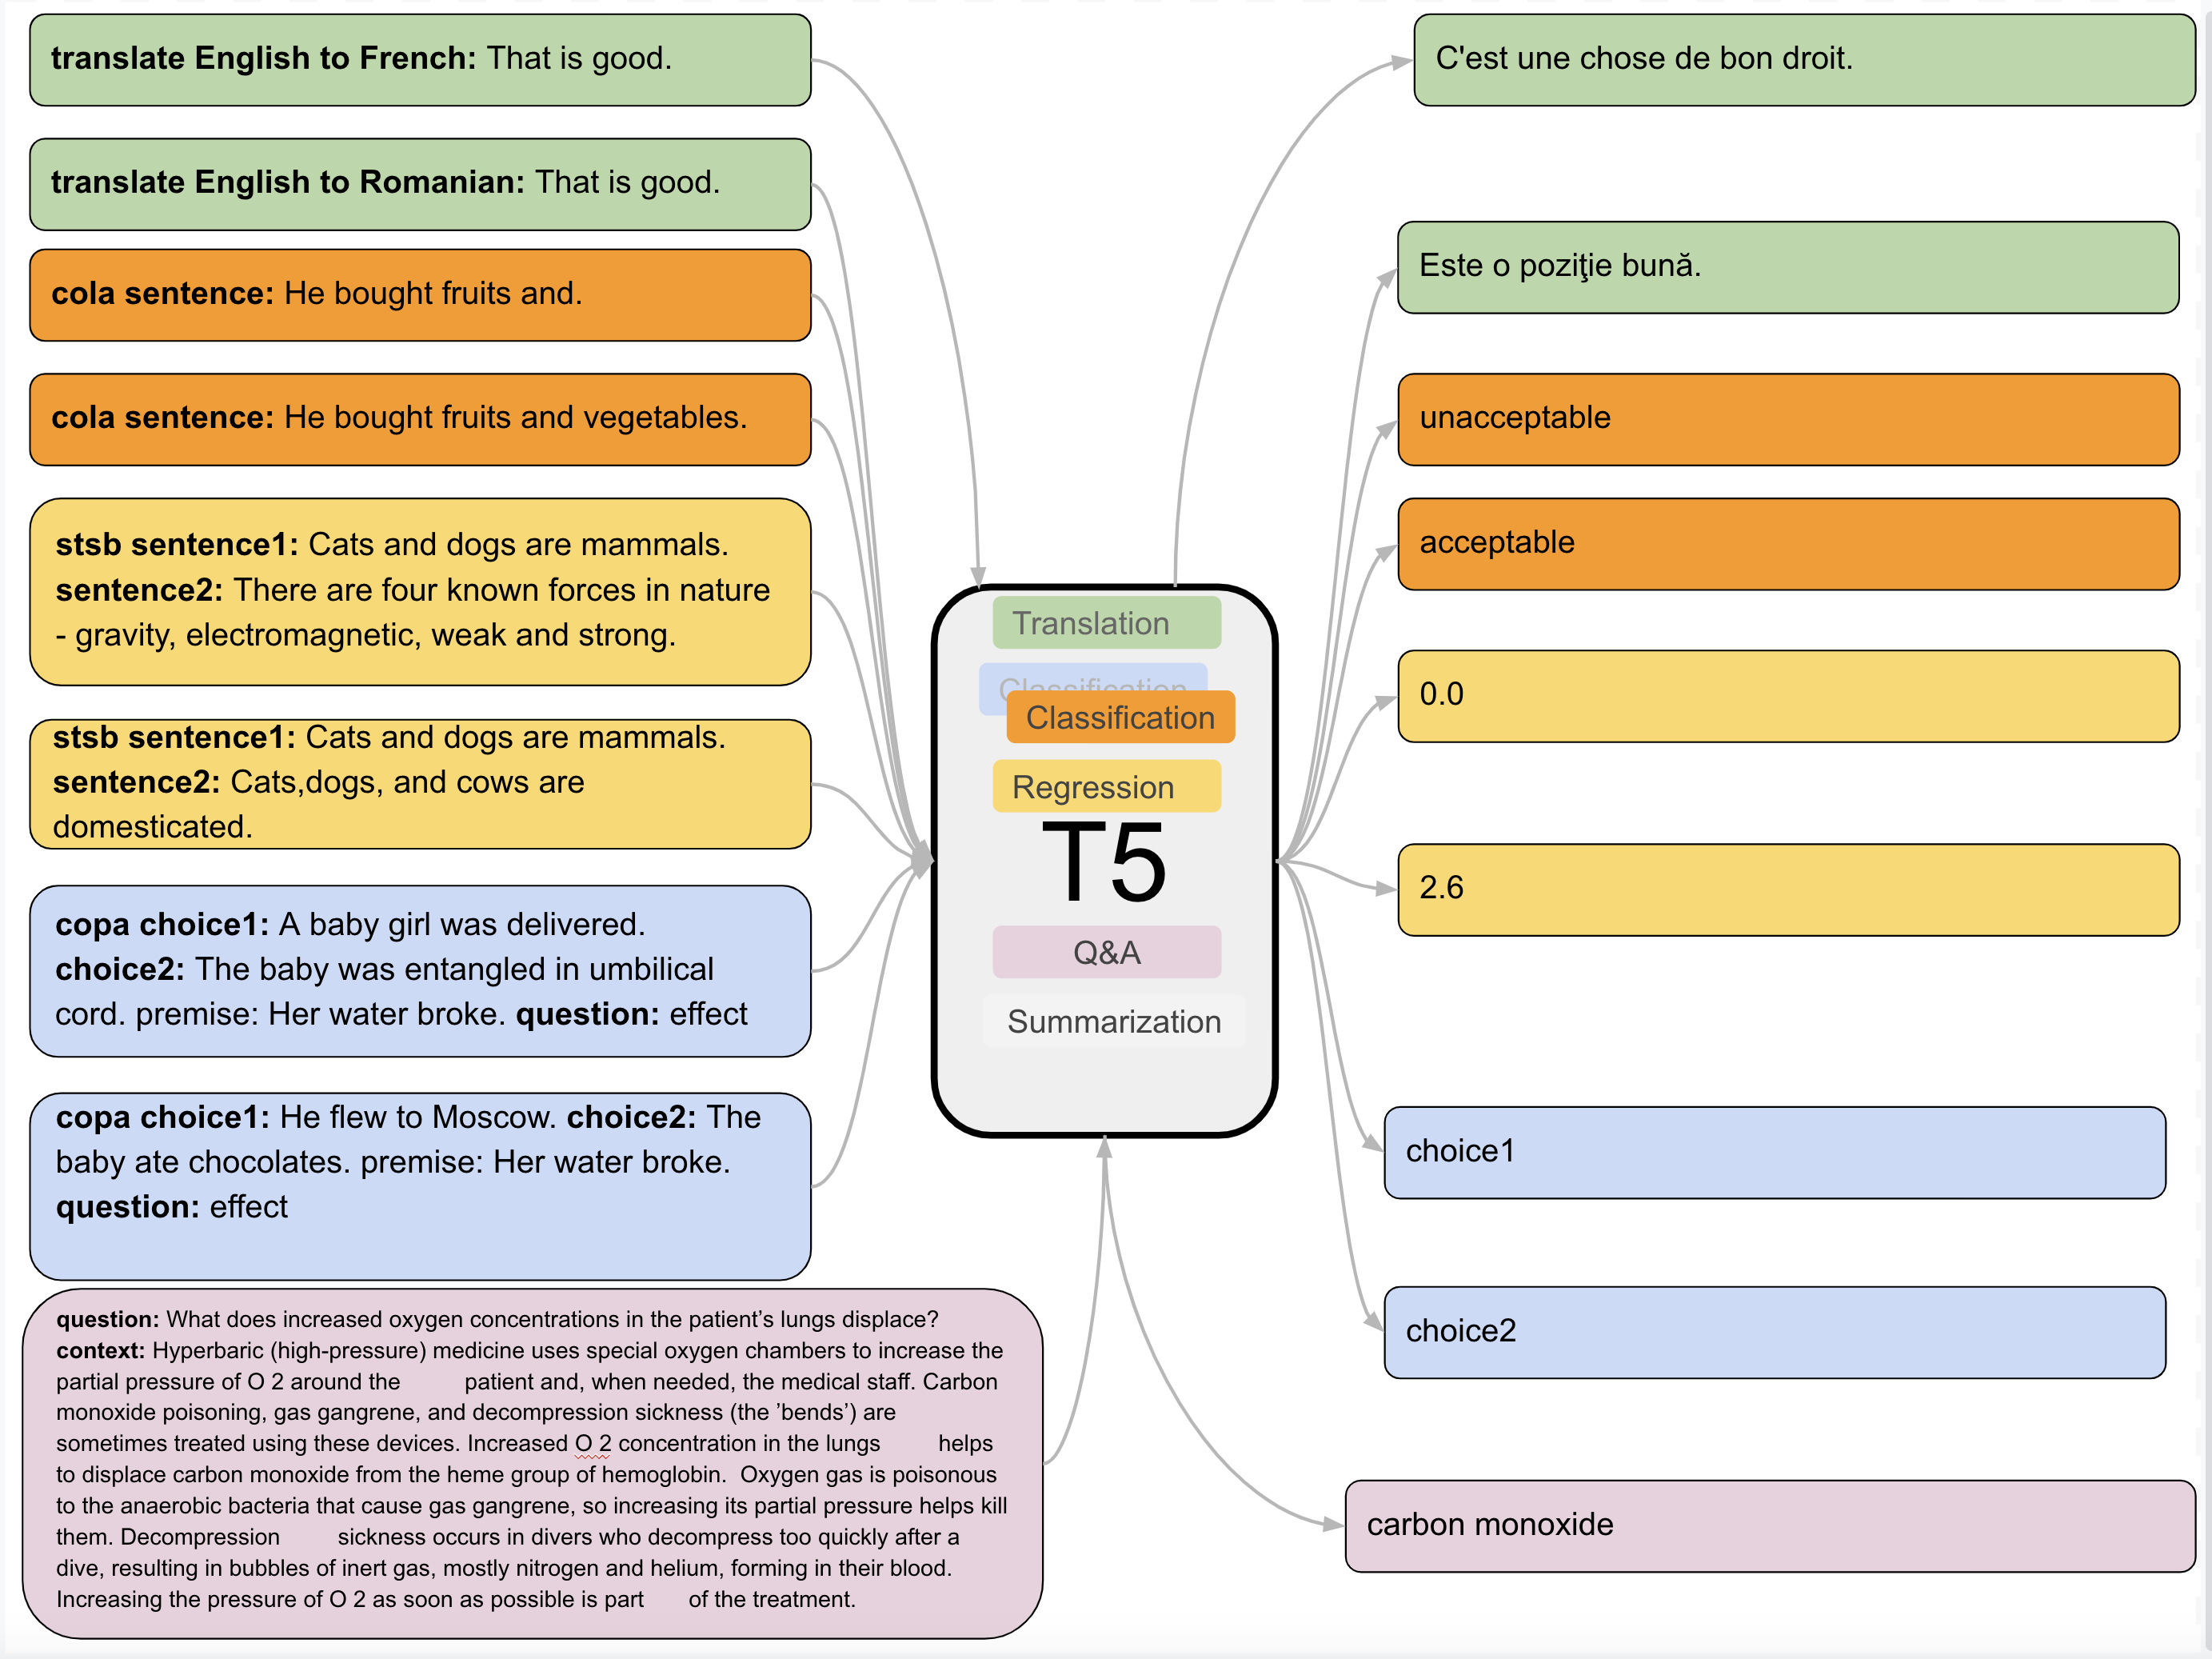
\includegraphics[width=\textwidth]{t5.png}}
\vfill
\onslide<2>{Translate:\vspace{-7mm}
  \begin{center}
  \fbox{Dave Grossman and Jack Thompson argue that violent games are harmful}
  
  $\downarrow$
  
  \fbox{Dave Grossman og Jack Thompson hævder, at voldsomme spil er skadelige}
  \end{center}
}
\vfill
\onslide<3>{
  Recognize entities:
  
  \fbox{\underline{Dave Grossman} and \underline{Jack Thompson} argue that violent games are harmful}
}
\vfill
\onslide<4>{ 
  Infer:
  \begin{center}
  \fbox{Violence in games hardens children to unethical acts}
  
  $\downarrow$ entails
  
  \fbox{Violent games are harmful}
  \end{center}
}
\end{frame}

\begin{frame}
\frametitle{Natural Language Processing in 2020: The Basics}
{\setbeamercovered{transparent}
1. Learn {\only<7>{\color{red}}\textit{representations}}:
\[{\only<5>{\color{red}}\Sigma^*}\to{\only<7>{\color{red}}\mathbb{R}^n}\]

\pause
2. Train classifiers:
\[{\only<7>{\color{red}}\mathbb{R}^n}\to {\only<6>{\color{red}}Y}\]

\pause
3. Deploy:
\[{\only<5>{\color{red}}\Sigma^*}\to {\only<6>{\color{red}}Y}\]

\pause
  \begin{center}
  \begin{adjustbox}{padding=1ex 1ex 1ex 1ex,frame,margin=1ex 1ex 1ex 1ex,minipage=[r][6ex][b]{.7\textwidth}}
  	\centering\rm\only<5>{\color{red}}\small
  	Violence in games hardens children to unethical acts \\ ? \\ Violent games are harmful
  \end{adjustbox}
  
  $\downarrow$
  
  {\only<7>{\color{red}}
  \begin{tikzpicture}
  \def\w{5};
  \draw (.5,7pt) arc[radius=7pt,start angle= 90,end angle=270];
  \draw (.5,-7pt) -- (\w+.5,-7pt);
  \draw (.5,7pt) -- (\w+.5,7pt);
  \draw (\w+.5,7pt) arc[radius=7pt,start angle=90,end angle=-90];
  \foreach \x in {1,...,\w}{
    \node[draw,radius=5pt,circle] at (\x,0) {};
  }
  \end{tikzpicture}}
  
  $\downarrow$
  
  {\tt\only<6>{\color{red}}entailment}
  \end{center}
}
\only<8>{
\begin{textblock*}{7cm}(3cm,0.8\textheight)
\begin{exampleblock}{}
\textit{Representation} = vector of real numbers?
\end{exampleblock}
\end{textblock*}}
\end{frame}

\newcommand{\mask}[2]{\alt<#1>{\fbox{\textbf{\color{red}?}}}{#2}}

\begin{frame}
\frametitle{Learning from plain text: masked language modeling}
\textrm{\mask{4}{Which} \mask{2}{Sesame} \mask{3}{Street} \mask{1}{character} \mask{5}{is} \mask{6}{your} \mask{7}{favorite}}

\vfill
\onslide<8>{
\textit{BERT} (Bidirectional Encoder Representations from Transformers):
\begin{itemize}
\item Trained on 16GB of text.
\item 16 TPU chips for 4 days.
\end{itemize}

\vfill

\url{https://demo.allennlp.org/masked-lm}
}

\vspace{-3cm}
\begin{flushright}

\includegraphics[width=.4\textwidth]{sesame.jpg}
\end{flushright}
\end{frame}

\begin{frame}
\frametitle{What can we teach computers to do with language?}
    Identify relations between concepts (\textbf{parsing}, various frameworks):

    \begin{adjustbox}{center}
    \begin{dependency}[line width=2pt,label style={line width=.5pt,draw=black}]
    \begin{deptext}
        Dave  \& Grossman \& and   \& Jack  \& Thompson \& argue \& that  \& violent \& games \& are \& harmful \& .     \\
	\end{deptext}
	\depedge{6}{1}{nsubj}
	\depedge{1}{2}{flat}
	\depedge{4}{3}{cc}
	\depedge{1}{4}{conj}
	\depedge{4}{5}{flat}
	\deproot[edge unit distance=3em]{6}{root}
	\depedge{11}{7}{mark}
	\depedge{9}{8}{amod}
	\depedge{11}{9}{nsubj}
	\depedge{11}{10}{cop}
	\depedge{6}{11}{ccomp}
	\depedge{6}{12}{punct}
    \end{dependency}
    \end{adjustbox}
\end{frame}

\begin{frame}
\setbeamercovered{transparent}
\frametitle{Breaking it down}
\small
[Meaning]\textit{,} [Representation] and [Parsing] \\
1. What we mean, 2. How to represent (something), 3. How to parse (something)

\pause
\vfill
or
\vfill

[Meaning Representation] and [Parsing] \\
1. How to represent what we mean, 2. How to parse (something)

\pause
\vfill
or 
\vfill

[Meaning [Representation and Parsing]] \\
1. How to represent what we mean, 2. How to parse what we mean

\pause
\vfill
or 
\vfill

[Meaning Representation] and [Parsing \textit{(to Meaning Representation)}] \\
1. How to represent what we mean, 2. How to parse (1)
\end{frame}

\begin{frame}
\frametitle{Meaning Representation}
{\only<3>{\color{red}Universal Conceptual Cognitive Annotation (UCCA):}}

\begin{adjustbox}{center}
            \begin{tikzpicture}[sibling distance=1mm,
                    frontier/.style={distance from root=28mm},
                    every node/.append style={font=\rmfamily},
            	    every circle node/.append style={fill=Indigo}]
                \begin{scope}[edge from parent path={(\tikzparentnode.center)
                	.. controls +(0,-.25) and +(0,.25) .. (\tikzchildnode.north)}]
                \Tree [.\node [circle] (root u) {};
                  [.\node [circle](Violence in video games u) {};
                    \edge node [auto=right]{}; \node (Violence u) {Violence};
                    \edge node [auto=right]{}; \node (in u) {in};
                    \edge node[auto=left]{};
                    [.\node [circle](video games u) {};
                      \edge node[auto=right]{}; \node (video u) {video};
                      \edge node[auto=right]{}; \node (games u) {games};
                    ]
                  ]
                  \edge node[auto=right]{}; \node (hardens u) {hardens};
                  \edge node[auto=right]{}; \node (children u) {children};
                  \edge node[auto=left]{};
                  [.\node [circle](to unethical acts u) {};
                    \edge node[auto=right]{}; \node (to u) {to};
                    \edge node[auto=left]{}; \node (unethical u) {unethical};
                    \edge node[auto=left]{}; \node (acts u) {acts};
                  ]
                ]
                \draw[dashed] (Violence in video games u) to[out=0,in=150] node[auto] {} (children u);
                \end{scope}
                \onslide<2->{
                \begin{scope}[grow'=up,xshift=-5mm,yshift=-62mm, sibling distance=2mm,
                    level 1/.style={sibling distance=4mm},
                    edge from parent path={(\tikzparentnode.center) ..
                    controls +(0,.25) and +(0,-.25) .. (\tikzchildnode.south)}]
                \Tree [.\node [circle] (root d) {};
                  [.\node [circle](Violence in video games d) {};
                    \edge node [auto=right]{}; \node (Violence d) {Vold};
                    \edge node [auto=right]{}; \node (in d) {i};
                    \edge node[auto=left]{};
                    \edge node[auto=right]{}; \node (video games d) {videospil};
                  ]
                  \edge node[auto=right]{}; \node (hardens d) {hærder};
                  \edge node[auto=right]{}; \node (children d) {børn};
                  \edge node[auto=left]{};
                  [.\node [circle](to unethical acts d) {};
                    \edge node[auto=right]{}; \node (to d) {til};
                    \edge node[auto=left]{}; \node (unethical d) {uetiske};
                    \edge node[auto=left]{}; \node (acts d) {handlinger};
                  ]
                ]
                \draw[dashed] (Violence in video games d) to[out=-15,in=-150] node[above] {} (children d);
                \end{scope}
                }
%                \onslide<3>{
%                  \begin{scope}[dashed,thick]
%                    \draw[DarkRed] (Violence u) to[out=-45,in=135] (Violence d);
%                    \draw[DarkGreen] (video games u) to[out=-90,in=100] (video games d);
%                    \draw[DarkBlue] (hardens u) -- (hardens d);
%                    \draw[orange] (children u) to[out=-30,in=90] (children d);
%                    \draw[magenta] (to unethical acts u) to[out=-90,in=70] (to unethical acts d);
%                  \end{scope}
%                }
            \end{tikzpicture}
\end{adjustbox}
\end{frame}

\def\exucca{
\begin{tikzpicture}[level distance=2cm, sibling distance=25mm, ->, draw=Indigo, thick]
    \node[font=\bf\sffamily\Huge,Indigo] at (-3,0) {UCCA};
    \node (ROOT) [fill=Indigo, circle] {}
      child {node (While) {While} edge from parent node[left] {L\;}}
      child {node (playing) [fill=Indigo, circle] {}
      {
        child {node {playing} edge from parent node[left] {P}}
      } edge from parent node[left] {H} }
      child {node {,} edge from parent node[right] {U}}
      child {node (learn) [fill=Indigo, circle] {}
      {
        child {node (children) {children} edge from parent node[left] {A}}
        child {node {learn} edge from parent node[left] {P}}
        child {node [fill=Indigo, circle] {}
        {
          child {node {about} edge from parent node[left] {R}}
          child {node {themselves} edge from parent node[left] {C}}
        } edge from parent node[left] {A} }
      } edge from parent node[right] {H} }
      ;
    \draw[dashed,->] (playing) to node [auto] {A} (children);
\end{tikzpicture}
}
\def\examr{
\begin{tikzpicture}[thick]
\node[font=\bf\sffamily\Huge,DarkGreen] at (0,1) {AMR};
\graph[layered layout, sibling distance=4cm, layer distance=2cm, nodes={ellipse,draw=DarkGreen}, edges={nodes={sloped}, DarkGreen}]{
a0[as={learn-01}];
a1[as={child}];
a5[as={during}];
a6[as={play-01}];

a0 ->  ["ARG0"' above] a1;
a0 ->  ["time"' above] a5;
a5 ->  ["op1"' above] a6;
};
\draw[->, above, DarkGreen] (a6) to node[sloped] {ARG0} (a1);
\draw[->, above, DarkGreen] (a0) to[out=180,in=90] node[sloped] {ARG1} (a1);
\end{tikzpicture}
}
\def\exdm{
    \begin{minipage}{.01\textwidth}
      \begin{tikzpicture}
        \node[font=\bf\sffamily\Large,DarkRed] {DM};
      \end{tikzpicture}
    \end{minipage}
    \begin{minipage}{.6\textwidth}
        \rmfamily
        \scalebox{.7}{
\begin{dependency}[theme=simple,edge style={-{Latex[length=2mm]}, color=DarkRed},
            text only label, label style={above, color=DarkRed, font=\bf\ttfamily}, font=\small, thick]
    \begin{deptext}[column sep=1em,ampersand replacement=\^]
	While \^ playing \^ , \^ children \^ learn \^ about \^ themselves \\
    \end{deptext}
    \deproot{5}{top}
    \depedge{1}{2}{ARG2}
    \depedge{1}{5}{ARG1}
    \depedge{5}{4}{ARG1}
    \depedge{6}{5}{ARG1}
    \depedge{6}{7}{ARG2}
\end{dependency}
    }
    \end{minipage}
}

\begin{frame}
    \frametitle{Many meaning representation frameworks exist}

      \begin{flushright}
        \scalebox{.6}{\exucca}
      \end{flushright}
    
    \vspace{-23mm}
    
    \scalebox{.6}{\examr}
    \vspace{-15mm}
    
    \begin{flushright}
	\exdm
    \end{flushright}
\end{frame}


\begin{frame}
\frametitle{Parsing}

\textit{A Transition-Based Directed Acyclic Graph Parser for UCCA} (2017)

\pause

\centering
\scalebox{.8}{
\begin{tikzpicture}[level distance=15mm, sibling distance=2cm, ->, thick,
    every node/.append style={font=\rmfamily},
    edge from parent path={(\tikzparentnode.center) -- (\tikzchildnode.north)}]
    \node(ROOT)[fill=black, circle] at (3,0) {}
      child {node (They) {They} edge from parent node [left] {A}}
      child {node (thought) {thought} edge from parent node [left] {P}}
      child {node (abouttakingashortbreak) [fill=blue, circle] {} 
      { 
        child {node (to) {about} edge from parent node [right] {R}}
        child {node (takingabreak) [fill=red, circle] {}
        {
          child {node (take) {taking} edge from parent node [above] {F}}      
          child {node (a) {a} edge from parent node [right] {F}} 
          child {node (short) {short} edge from parent [draw=none]}
          child {node (break) {break} edge from parent node [above] {C}}  
        } edge from parent [draw=none]}
      } edge from parent [draw=none]}
      ;
    \draw(abouttakingashortbreak) to node [left] {P} (takingabreak); 
    \draw(ROOT) to node [left] {A} (abouttakingashortbreak);
    \draw[bend left,dashed] (abouttakingashortbreak) to node [auto] {A} (They);
    \draw[bend left] (abouttakingashortbreak) to node [auto] {D} (short);
\end{tikzpicture}}
\[\Updownarrow\]
\begin{flushleft}
\footnotesize
\textsc{Shift}, \textsc{Right-Edge$_A$}, \textsc{Shift}, \textsc{Swap}, \textsc{Right-Edge$_P$}, \textsc{Reduce}, \textsc{Shift}, \textsc{Shift}, \textsc{Node$_R$}, \textsc{Reduce}, \textsc{Left-Remote$_A$}, \textsc{Shift}, \textsc{Shift}, \textsc{Node$_C$}, \textsc{Reduce}, \textsc{Shift}, \textsc{Right-Edge$_P$}, \textsc{Shift}, \textsc{Right-Edge$_F$}, \textsc{Reduce}, \textsc{Shift}, \textsc{Swap}, \textsc{Right-Edge$_D$}, \textsc{Reduce}, \textsc{Swap}, \textsc{Right-Edge$_A$}, \textsc{Reduce}, \textsc{Reduce}, \textsc{Shift}, \textsc{Reduce}, \textsc{Shift}, \textsc{Right-Edge$_C$}, \textsc{Finish}
\end{flushleft}
\end{frame}

\begin{frame}
\frametitle{TUPA: Transition-based UCCA Parser}

Parses text $w_1 \ldots w_n$ to graph $G$ incrementally by applying transitions to the parser state,
consisting of: stack, buffer and constructed graph.

\pause
\vfill
Initial state:
\scalebox{.9}{
\begin{tikzpicture}[xscale=1.4,every node/.append style={font=\rmfamily,
                    anchor=west,text height=.6ex,text depth=0}, circle]
    \draw[xstep=1,ystep=.5,color=gray] (-.01,0) grid (1,.5);
    \node[style={font=\sffamily}] at (-.1,.8) {stack};
    \node[fill=black] at (.3,.25) {};
    \draw[xstep=1,ystep=.5,color=gray] (2,0) grid (9,.5);
    \node[style={font=\sffamily}] at (8,.8) {buffer};
    \node at (2,.2) {\small They};
    \node at (3,.2) {\small thought};
    \node at (4,.2) {\small about};
    \node at (5,.2) {\small taking};
    \node at (6,.2) {\small a};
    \node at (7,.2) {\small short};
    \node at (8,.2) {\small break};
\end{tikzpicture}}

\vfill
\pause
Transitions:

\{\textsc{Shift, Reduce, {\color{blue}Node$_X$}, Left-Edge$_X$, Right-Edge$_X$,}\\
\hspace{5mm}\textsc{{\color{orange}Left-Remote$_X$}, {\color{orange}Right-Remote$_X$}, {\color{red}Swap}, Finish}\}
\end{frame}

\begin{frame}
\frametitle{Example: TUPA Transition Sequence}
\begin{minipage}[t][8mm][t]{\textwidth}
    $\Rightarrow$\textsc{
        \only<1>{Shift}\only<2>{Right-Edge$_A$}\only<3>{Shift}\only<4>{Swap}\only<5>{Right-Edge$_P$}\only<6>{Reduce}\only<7>{Shift}\only<8>{Shift}\only<9>{Node$_R$}\only<10>{Reduce}\only<11>{Shift}\only<12>{Left-Remote$_A$}\only<13>{Shift}\only<14>{Node$_C$}\only<15>{Reduce}\only<16>{Shift}\only<17>{Right-Edge$_P$}\only<18>{Shift}\only<19>{Right-Edge$_F$}\only<20>{Reduce}\only<21>{Shift}\only<22>{Swap}\only<23>{Right-Edge$_D$}\only<24>{Reduce}\only<25>{Swap}\only<26>{Right-Edge$_A$}\only<27>{Reduce}\only<28>{Reduce}\only<29>{Shift}\only<30>{Reduce}\only<31>{Shift}\only<32>{Right-Edge$_C$}\only<33>{Finish}
    }
\end{minipage}

\vfill

\scalebox{.9}{
\begin{tikzpicture}[xscale=1.4,every node/.append style={font=\rmfamily, thick,
                    anchor=west,text height=.6ex,text depth=0}]
    \begin{scope}[style={font=\sffamily}]
      \node at (-.1,.8) {stack};
      \node at (8,  .8) {buffer};
    \end{scope}
    \begin{scope}[xstep=1,ystep=.5,color=red,line width=1pt]
      \only<31>    \draw (-.01,0) grid (1,.5);
      \only<1,7>   \draw (.99, 0) grid (2,.5);
      \only<2,5,26>\draw (-.01,0) grid (2,.5);
      \only<3,8,11>\draw (1.99,0) grid (3,.5);
      \only<13,16> \draw (2.99,0) grid (4,.5);
      \only<18,21> \draw (3.99,0) grid (5,.5);
      \only<17>    \draw (1.99,0) grid (4,.5);
      \only<19>    \draw (2.99,0) grid (5,.5);
      \only<4>     \draw (3,   0) grid (4,.5);
      \only<9>     \draw (4,   0) grid (5,.5);
      \only<14>    \draw (5,   0) grid (6,.5);
      \only<22>    \draw (7,   0) grid (8,.5);
      \only<25>    \draw (6,   0) grid (7,.5);
      \only<23>    \draw (1.99,0) grid (4,.5);
      \only<32>    \draw (-.01,0) grid (2,.5);
      \only<12>    \draw (.99, 0) grid (3,.5);
    \end{scope}
    \begin{scope}[xstep=1,ystep=.5,color=gray]
      \only<6,27,29,31->         \draw (-.01,0) grid (1, .5);
      \only<-2,4-5,7,10,25-26,33>\draw (-.01,0) grid (2, .5);
      \only<3,8-9,11-12,15,24>   \draw (-.01,0) grid (3, .5);
      \only<13-14,16-17,20,22-23>\draw (-.01,0) grid (4, .5);
      \only<18-19,21>            \draw (-.01,0) grid (5, .5);
      \only<-2,4-6>              \draw (3,   0) grid (9,.5);
      \only<3,5-7,9-10>          \draw (4,   0) grid (9,.5);
      \only<8,11-12,14-15>       \draw (5,   0) grid (9,.5);
      \only<13,16-17,25-28>      \draw (6,   0) grid (9,.5);
      \only<18-20,22-24,29-30>   \draw (7,   0) grid (9,.5);
      \only<21,31>               \draw (8,   0) grid (9,.5);
    \end{scope}
    \begin{scope}[xstep=.1,ystep=.5,color=gray]
      \only<28,30> \draw (-.01,0) grid (.1,.5);
      \only<32->   \draw (8.89,0) grid (9.01,.5);
    \end{scope}
    \only<-27>      \node[fill=black, circle] at (.3, .25) {};
    \only<25-26>    \node[fill=blue,  circle] at (1.3,.25) {};
    \only<11-24>    \node[fill=blue,  circle] at (2.3,.25) {};
    \only<31->      \node[fill=red,   circle] at (.3, .25) {};
    \only<16-21>    \node[fill=red,   circle] at (3.3,.25) {};
    \only<9-10>     \node[fill=blue,  circle] at (4.3,.25) {};
    \only<14-15>    \node[fill=red,   circle] at (5.3,.25) {};
    \only<22-30>    \node[fill=red,   circle] at (7.3,.25) {};
    \only<29>       \node at (0,.2) {\small They};
    \only<1-3,7-24> \node at (1,.2) {\small They};
    \only<4-5>      \node at (1,.2) {\small thought};
    \only<3>        \node at (2,.2) {\small thought};
    \only<8-9>      \node at (2,.2) {\small about};
    \only<13-14>    \node at (3,.2) {\small taking};
    \only<18-19>    \node at (4,.2) {\small a};
    \only<21>       \node at (4,.2) {\small short};
    \only<22-23>    \node at (3,.2) {\small short};
    \only<32->      \node at (1,.2) {\small break};
    \only<4-6>      \node at (3,.2) {\small They};
    \only<25-28>    \node at (6,.2) {\small They};
    \only<-2>       \node at (3,.2) {\small thought};
    \only<-7>       \node at (4,.2) {\small about};
    \only<-12>      \node at (5,.2) {\small taking};
    \only<-17>      \node at (6,.2) {\small a};
    \only<-20>      \node at (7,.2) {\small short};
    \only<-31>      \node at (8,.2) {\small break};
\end{tikzpicture}}
\vfill
\fbox{
\begin{tikzpicture}[level distance=14mm, sibling distance=26mm, ->,
    every node/.append style={font=\rmfamily},
    edge from parent/.append style={nodes={font=\scriptsize}},
    edge from parent path={(\tikzparentnode.center) -- (\tikzchildnode.north)}]
    \node[anchor=west,style={font=\sffamily}] at (0,0) {graph};
    \node(ROOT)[fill=black, circle, visible on=<1->] at (3,0) {}
      child [visible on=<2->,alt=<2>{draw=red}{}] {node (They) {They} edge from parent node [left] {A}}
      child [visible on=<5->,alt=<5>{draw=red}{}] {node (thought) {thought} edge from parent node [left] {P}}
      child [visible on=<9->] {node (abouttakingashortbreak) [fill=blue, circle] {}
      {
        child [visible on=<9->,alt=<9>{draw=red}{}] {node (to) {about} edge from parent node [right] {R}}
        child [visible on=<14->] {node (takingabreak) [fill=red, circle] {}
        {
          child [visible on=<14->] {node (take) {taking} edge from parent node [above] {F}}
          child [visible on=<19->,alt=<19>{draw=red}{}] {node (a) {a} edge from parent node [right] {F}}
          child [visible on=<23->,alt=<23>{draw=red}{}] {node (short) {short} edge from parent [draw=none]}
          child [visible on=<32->,alt=<32>{draw=red}{}] {node (break) {break} edge from parent node [above] {C}}
        } edge from parent [draw=none]}
      } edge from parent [draw=none]}
      ;
    \draw[visible on=<17->,alt=<17>{draw=red}{}] (abouttakingashortbreak) to node [left] {\scriptsize P} (takingabreak);
    \draw[visible on=<26->,alt=<26>{draw=red}{}] (ROOT) to node [left] {\scriptsize A} (abouttakingashortbreak);
    \draw[bend left,dashed, visible on=<12->,alt=<12>{draw=red}{}] (abouttakingashortbreak) to node [auto] {\scriptsize A} (They);
    \draw[bend left, visible on=<23->,alt=<23>{draw=red}{}] (abouttakingashortbreak) to node [auto] {\scriptsize D} (short);
\end{tikzpicture}}
\end{frame}

\begin{frame}
\frametitle{TUPA model}
Learns to predict next transition based on current state.

\centering
\fbox{\scalebox{.65}{
\begin{minipage}{.6\textwidth}
\begin{tikzpicture}[xscale=1.3,every node/.append style={font=\rmfamily}]
    \node[anchor=west,style={font=\sffamily}] at (-1,.25){stack};
    \draw[xstep=1,ystep=.5,color=gray] (-.01,0) grid (4,.5);
    \node[fill=black, circle] at (.5,.25) {};
    \node[fill=blue, circle] at (2.5,.25) {};
    \node[anchor=west] at (1,.25) {\small They};
    \node[anchor=west] at (3,.25) {\small taking};
\end{tikzpicture}

\vspace{1cm}
\begin{tikzpicture}[xscale=1.3,every node/.append style={font=\rmfamily}]
    \node[anchor=west,style={font=\sffamily}] at (-1,.25){buffer};
    \draw[xstep=1,ystep=.5,color=gray] (-.01,0) grid (4,.5);
    \node[fill=red, circle] at (.5,.25) {};
    \node[anchor=west] at (1,.25) {\small a};
    \node[anchor=west] at (2,.25) {\small short};
    \node[anchor=west] at (3,.25) {\small break};
\end{tikzpicture}
\end{minipage}
\begin{minipage}{.4\textwidth}
\scalebox{.65}{
\begin{tikzpicture}[xscale=1.5,level distance=1cm, sibling distance=12mm, ->,
    every node/.append style={font=\rmfamily,
                    anchor=west,text height=.6ex,text depth=0},
    edge from parent/.append style={nodes={font=\scriptsize}},
    edge from parent path={(\tikzparentnode.center) -- (\tikzchildnode.north)}]
    \node[anchor=west,style={font=\sffamily}] at (3,0) {graph};
    \draw[color=gray] (.2,.3) rectangle (3.9,-3.2);
    \node(ROOT)[fill=black, circle] at (1.2,0) {}
      child {node (They) {They} edge from parent node [left] {A}}
      child {node {thought} edge from parent node [left] {P}}
      child {node (abouttakingashortbreak) [fill=blue, circle] {}
      {
        child {node {about} edge from parent node [left] {R}}
        child {node (takingabreak) [fill=red, circle] {}
        {
          child {node {taking} edge from parent node [above] {F}}
          child [opacity=0] {node {a} edge from parent node [right] {F}}
          child [opacity=0] {node (short) {short} edge from parent [draw=none]}
          child [opacity=0] {node {break} edge from parent node [right] {C}}
        } edge from parent [draw=none]}
      } edge from parent [draw=none]}
      ;
\end{tikzpicture}
}
\end{minipage}
}}

\scalebox{.65}{
\begin{tikzpicture}[->,every node/.append style={anchor=north,text height=2ex,text depth=0}]
    \tiny
    \tikzstyle{main}=[circle, minimum size=7mm, draw=black!80, node distance=12mm]
    \foreach \i/\word in {1/{They},3/{thought},5/{about},7/{taking},9/{a},11/{short},13/{break}} {
        \node (x\i) at (\i,-1.3) {\Large\textrm\word};
        \node[main, fill=white!100] (h\i) at (\i,0) {};
        \path (x\i) edge (h\i);
        \node[main, fill=white!100] (i\i) at (\i.5,.8) {};
        \path (x\i) edge [bend right] (i\i);
        \node[main, fill=white!100] (l\i) at (\i.5,2.3) {};
        \path (h\i) edge [bend left] (l\i);
        \path (i\i) edge (l\i);
        \node[main, fill=white!100] (k\i) at (\i,3.1) {};
        \path (i\i) edge [bend left] (k\i);
        \path (h\i) edge [bend left] (k\i);
    }
    \foreach \current/\next in {1/3,3/5,5/7,7/9,9/11,11/13} {
        \path (h\current) edge (h\next);
        \path (i\next) edge (i\current);
        \path (l\current) edge (l\next);
        \path (k\next) edge (k\current);
    }
    \node[main, fill=white!100] (mlp) at (7,4.6) {};
    \foreach \i in {1,5,7,9} {
        \path (l\i) edge (mlp);
        \path (k\i) edge (mlp);
    }
    \coordinate (state) at (10.5,6.5);
    \path (state) edge [bend left] (mlp);
    \node (transition) at (7,5.8) {\large\textsc{Node}$_C$};
    \path (mlp) edge (transition);
\end{tikzpicture}
}
\end{frame}


\begin{frame}
    \frametitle{Sharing for better generalization}
    
    \textit{Multitask Parsing Across Semantic Representations} (2018)
    
    \vfill
    
    \begin{minipage}{.06\pagewidth}
    \scalebox{8}{\{}
    \end{minipage}
    \begin{minipage}{.27\pagewidth}
    \scalebox{.32}{\exucca}
    \end{minipage}
    \begin{minipage}{.22\pagewidth}
    \scalebox{.5}{\examr}
    \end{minipage}
    \begin{minipage}{.23\pagewidth}
    \scalebox{.5}{\exdm}
    \end{minipage}
    \begin{minipage}{.06\pagewidth}
    \scalebox{8}{\}}
    \end{minipage}
    
    \vfill
    \pause
    
    Improved UCCA parsing in English, French and German.
\end{frame}

\begin{frame}
\frametitle{Multilingual semantic parsing from grounding in Wikidata}
Build knowledge graph search queries from natural language expressions \\
using methods from meaning representation parsing \\
and reinforcement learning.

\vfill

\begin{textblock*}{64mm}(32mm,0.33\textheight)
\begin{exampleblock}{}
impressionist painters \\
18th-century American poets \\
\ldots
\end{exampleblock}
\end{textblock*}


\includegraphics[width=.3\textwidth]{wikipedia.png}\hfill

\includegraphics[width=.3\textwidth]{640px-Wikidata-logo-en.png}
\end{frame}

\begin{frame}
\frametitle{Meaning representation for machine translation}
(Simplified) Vauquois triangle:

\begin{center}
\begin{tikzpicture}[line width=2pt]
\graph[tree layout, sibling distance=6cm, layer distance=3cm, nodes={rectangle,draw=DarkBlue,align=center}, edges={nodes={sloped}, DarkRed}]{
a2[as={Interlingua}];
a1[as={Source meaning \\ representation}];
a0[as={Source text}];
b1[as={Target meaning \\ representation}];
b0[as={Target text}];

(a0) -> ["parsing"' above] (a1);
(a2) <- [out=180,in=90] (a1);
(b0) <- ["generation"' above] (b1);
(a2) -> [out=0,in=90] (b1);
};
\pause
\graph{
(a0) -> [dashed] (b0);
};
\pause
\graph{
(a1) -> [dashed] (b1);
};
\pause
\graph{
(a1) -> [dashed] (b0);
};
\end{tikzpicture}
\end{center}
\end{frame}

\begin{frame}
\frametitle{Next steps}
\begin{itemize}
 \item Is meaning representation necessary for language understanding?\pause
 \begin{itemize}
 \item As an infrastructure for better deep learning\pause
 \item As an interpretation method for probing linguistic knowledge\pause
 \item {\only<9>{\color{red}}As a goal in itself---e.g., for querying knowledge bases}\pause
 \end{itemize}
 \vfill
 \item Can we make NLP methods robust to new domains and languages?\pause
 \begin{itemize}
 \item By simply experimenting with more diverse data\pause
 \item By principled multitask learning\pause
 \item By better understanding generalization
 \end{itemize}
\end{itemize}
\end{frame}

\begin{frame}
\frametitle{Shared tasks: parsing competitions}
\textit{SemEval 2019 Task 1: Cross-lingual Semantic Parsing with UCCA}

\begin{minipage}{.6\textwidth}
\begin{itemize}
\item 3 languages.
\item 8 teams from 6 countries.
\end{itemize}
\end{minipage}
\hfill
\begin{minipage}{.1\textwidth}
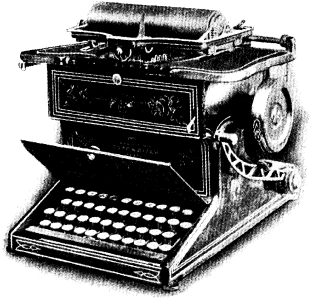
\includegraphics[width=\textwidth]{type_writer2.png}
\end{minipage}

\pause
\vfill

\textit{MRP 2019: Cross-Framework Meaning Representation Parsing}

\begin{minipage}{.6\textwidth}
\begin{itemize}
\item 5 frameworks.
\item 18 teams from 8 countries.
\end{itemize}
\end{minipage}
\hfill
\begin{minipage}{.1\textwidth}

\includegraphics[width=\textwidth]{logo.png}
\end{minipage}

\pause
\vfill

soon...

\textit{MRP 2020}

\begin{minipage}{.6\textwidth}
\begin{itemize}
\item More frameworks.
\item 5 languages.
\end{itemize}
\end{minipage}
\hfill
\begin{minipage}{.1\textwidth}

\includegraphics[width=\textwidth]{logo.png}
\end{minipage}
\end{frame}

\begin{frame}[allowframebreaks]
\frametitle{References}
\bibliographystyle{plainnat}
\tiny\bibliography{references}
\end{frame}

\begin{frame}
\frametitle{Structural Properties}
\noindent
\centering
\begin{minipage}{.5\linewidth}{\centering
(1) {\color{blue} non-terminal nodes}

\scalebox{.8}{
  \begin{tikzpicture}[level distance=12mm, sibling distance=16mm, ->, thick,
      every node/.append style={midway},
      edge from parent/.append style={nodes={font=\scriptsize}}]
    \node (ROOT) [fill=blue, circle] {}
      child {node [fill=blue, circle] {}
      {
        child {node {John} edge from parent node[left] {C}}
        child {node {and} edge from parent node[left] {N}}
        child {node {Mary} edge from parent node[right] {C}}
      } edge from parent node[left] {A} }
      child {node {went} edge from parent node[left] {P}}
      child {node {home} edge from parent node[right] {A}}
      ;
  \end{tikzpicture}
  }}
\end{minipage}
\hfill
\begin{minipage}{.48\linewidth}{\centering
(2) {\color{red} discontinuity}

\scalebox{.8}{
  \begin{tikzpicture}[level distance=12mm, sibling distance=2cm, ->, thick,
      every node/.append style={midway},
      edge from parent/.append style={nodes={font=\scriptsize}}]
    \node (ROOT) [fill=black, circle] {}
      child {node {John} edge from parent node[left] {A}}
      child {node [fill=black, circle] {}
      {
      	child {node {gave} edge from parent node[left] {C}}
      	child {node (everything) {everything} edge from parent[white]}
      	child {node {up} edge from parent node[right] {C}}
      } edge from parent node[right] {P} }
      ;
    \draw[bend right,->,red,very thick] (ROOT) to[out=-20, in=180] node [left] {\scriptsize A} (everything);
  \end{tikzpicture}
  }}
\end{minipage}

\vfill
(3) {\color{orange} reentrancy}

\scalebox{.8}{
\begin{tikzpicture}[level distance=14mm, sibling distance=17mm, ->, thick,
    edge from parent/.append style={nodes={font=\scriptsize}}]
    \node (ROOT) [fill=black, circle] {}
      child {node (After) {After} edge from parent node[left] {L\;}}
      child {node (graduation) [fill=black, circle] {}
      {
        child {node {graduation} edge from parent node[left] {P}}
      } edge from parent node[left] {H} }
      child {node {,} edge from parent node[right] {U}}
      child {node (moved) [fill=black, circle] {}
      {
        child {node (John) {John} edge from parent node[left] {A}}
        child {node {moved} edge from parent node[left] {P}}
        child {node [fill=black, circle] {}
        {
          child {node {to} edge from parent node[left] {R}}
          child {node {Copenhagen} edge from parent node[right] {C}}
        } edge from parent node[right] {A} }
      } edge from parent node[right] {H} }
      ;
    \draw[dashed,->,orange,very thick] (graduation) to node [auto] {\scriptsize A} (John);
\end{tikzpicture}}
\end{frame}


\begin{frame}
\frametitle{Data Statistics}
\centering
\def\arraystretch{1.5}
\begin{tabular}{l|r|rrr|r}
    & \multicolumn{1}{c|}{Wiki} & \multicolumn{3}{c|}{20K} & \multicolumn{1}{c}{EWT} \\
    & \multicolumn{1}{c|}{en} & \multicolumn{1}{c}{en} & \multicolumn{1}{c}{fr} & \multicolumn{1}{c|}{de} & \multicolumn{1}{c}{en} \\
    \hline
    \# sentences&5,141&492&492&6,514&3,520 \\
    \# tokens&158,739&12,638&13,021&144,529&51,042 \\
    \hline
    \# {\color{blue} non-terminal nodes}&62,002&4,699&5,110&51,934&18,156 \\
    \% {\color{red}discontinuous}&1.71&3.19&4.64&8.87&3.87 \\
    \% {\color{orange}reentrant}&1.84&0.89&0.65&0.31&0.83 \\
    \hline
    \# edges&208,937&16,803&17,520&187,533&60,739 \\
    \% primary&97.40&96.79&97.02&97.32&97.32 \\
    \% remote&2.60&3.21&2.98&2.68&2.68
\end{tabular}
\end{frame}


\begin{frame}
\frametitle{Evaluation}
\begin{adjustbox}{frame,scale=.75,center}
    \begin{tikzpicture}[level distance=12mm, sibling distance=15mm, ->,
        every circle node/.append style={fill=black},
        edge from parent/.append style={nodes={font=\scriptsize}},
        edge from parent path={(\tikzparentnode.center) -- (\tikzchildnode.north)}]
      \tikzstyle{word} = [font=\rmfamily,color=black]
      \node at (0,.7) {True (human-annotated) graph};
      \node (ROOT) at (0,0) [circle] {}
        child {node (After) [word] {After} edge from parent node[left] {L}}
        child {node (graduation) [circle] {}
        {
          child {node [word] {graduation} edge from parent node[left] {P}}
        } edge from parent node[left] {H} }
        child {node [word] {,} edge from parent node[right] {U}}
        child {node (moved) [circle] {}
        {
          child {node (John) [word] {John} edge from parent node[left] {A}}
          child {node [word] {moved} edge from parent node[left] {P}}
          child {node [circle] {}
          {
            child {node [word] {to} edge from parent node[left] {R}}
            child {node [word] {Copenhagen} edge from parent node[right] {C}}
          } edge from parent node[right] {A} }
        } edge from parent node[right] {H} }
        ;
      \draw[dashed,->] (graduation) to node [auto] {\scriptsize A} (John);
      \node at (8,.7) {Automatically predicted graph for the same text};
      \node (ROOT_) at (7,0) [circle] {}
        child {node (After_) [word] {After} edge from parent node[left] {L}}
        child {node (graduation_) [circle] {}
        {
          child[alt=<2>{red}{}] {node [word] {graduation} edge from parent node[left] {S}}
        } edge from parent node[left] {H} }
        child {node [word] {,} edge from parent node[right] {U}}
        child {node (moved) [circle,xshift=3mm,yshift=-7mm] {}
        {
          child {node (John_) [word] {John} edge from parent node[left] {A}}
          child {node [word] {moved} edge from parent node[left] {P}}
          child[alt=<2>{red}{}] {node [word] {to} edge from parent node[left] {F}}
          child[alt=<2>{red}{}] {node (Copenhagen_) [word] {Copenhagen} edge from parent node[right] {A}}
        } edge from parent node[right] {H} }
        ;
      \draw[dashed,->] (graduation_) to node [auto] {\scriptsize A} (John_);
      \draw[bend left,dashed,->,alt=<2>{red}{}] (graduation_) to[in=90] node [auto] {\scriptsize A} (Copenhagen_);
    \end{tikzpicture}
\end{adjustbox}
\vfill

\begin{enumerate}
  \item Match primary edges between the graphs by terminal yield and label.
  \item Calculate \textbf{precision, recall and F1} scores.
  \item Repeat for remote edges.
\end{enumerate}

\pause
\vfill
\begin{adjustbox}{center}
    \begin{tabular}{c|c|c}
        \multicolumn{3}{l}{Primary} \\
        \textbf{P} & \textbf{R} & \textbf{F1} \\ \hline
        $\frac69=67\%$ & $\frac6{10}=60\%$ & 64\%
    \end{tabular}
    \hspace{1cm}
    \begin{tabular}{c|c|c}
        \multicolumn{3}{l}{Remote} \\
        \textbf{P} & \textbf{R} & \textbf{F1} \\ \hline
        $\frac12=50\%$ & $\frac11=100\%$ & 67\%
    \end{tabular}
\end{adjustbox}
\end{frame}

\end{document}
